%% Beamer template for the International Agency for Research on Cancer (IARC)
%% v1.0 by Nicolas Alcala (email: alcalan@fellows.iarc.fr)

\documentclass[compress]{beamer}
\usepackage{etex}

\mode<presentation>
{
 \usetheme{IARC}
}

\usepackage[english]{babel}
\usepackage{amssymb}
\usepackage{epsfig}
\usepackage{geometry}
\usepackage{wrapfig}
\usepackage{subfig}

\usepackage{graphics}
\usepackage{graphicx}
\usepackage{amsmath,supertabular,tabularx}
\usepackage{multirow}
\usepackage{color}
\usepackage{verbatim}
\usepackage{stmaryrd}
%%for graphs 
\usepackage{ifthen}
\usepackage{hyperref}
\hypersetup{
    colorlinks=true,
    linkcolor=white,
    filecolor=magenta,      
    urlcolor=cyan,
}
\usepackage{appendixnumberbeamer}
\usepackage[]{natbib}
\bibpunct{(}{)}{;}{author-year}{}{,} 

\beamerboxesdeclarecolorscheme{clair}{darkgray}{white}
\beamerboxesdeclarecolorscheme{beige}{beige}{white}

\definecolor{lightblue}{rgb}{0.1,0.9,0.9}
\definecolor{lightred}{rgb}{0.9,0.4,0.4}
\definecolor{darkgreen}{rgb}{0.1,0.6,0.1}
\definecolor{Lightgray}{rgb}{0.85,0.85,0.85}
\definecolor{lightgray}{rgb}{0.65,0.65,0.65}
\definecolor{darkgray}{rgb}{0.35,0.35,0.35}
\definecolor{normalblue}{rgb}{0.35,0.35,0.9}
\definecolor{darkgray2}{rgb}{0.90,0.90,0.90}
\definecolor{darkred}{rgb}{0.6,0.1,0.1}

\newcounter{meta}
\setcounter{meta}{0}
\renewcommand{\thefootnote}{\fnsymbol{footnote}}

%\captionsetup[subfigure]{labelformat=empty}


\newcommand*\textfbox[2][title]{%
  \begin{tabular}[b]{@{}c@{}}#1\\\fbox{#2}\end{tabular}
}

\newcommand*\textfboxbelow[2][title]{%
  \begin{tabular}[b]{@{}c@{}}\fbox{#2}\\#1\end{tabular}
}


\title[Short Title]{Title}
\author[Short Author name]{Author Name}
\institute{X group}
\date{\today}

\begin{document}

\begin{frame}
\titlepage

\end{frame}
 
\section{Introduction}

\begin{frame}

\textbf{A list:}
\begin{itemize}
\item An item
\item<2> An item that appears only on 2nd frame
\item<3-> An item that appears at 3rd frame
\item Another item
\end{itemize}

\end{frame}



\section{Section 1}

\subsection{Subsection title}

\begin{frame}

%% example page subdivision with minipage
\begin{minipage}{0.45\linewidth}
\begin{beamerboxesrounded}[scheme=beige,shadow=true]{\textbf{Box title in left minipage} }

\begin{footnotesize}
\textit{An enumeration example} \citep{bob2017}:
\begin{enumerate}
\item 1st item \hyperlink{SI1}{\beamerbutton{link to SI}}
\item 2nd item \href{run:example.txt}{(link to an external file)} 
\item 3nd item (\url{https://github.com/IARCbioinfo/})
\end{enumerate}
\end{footnotesize}
\end{beamerboxesrounded}

\end{minipage}
\hspace*{3mm}
\begin{minipage}{0.50\linewidth}
Display some plot on right minipage only at given frame:

\onslide<3->{\begin{center}
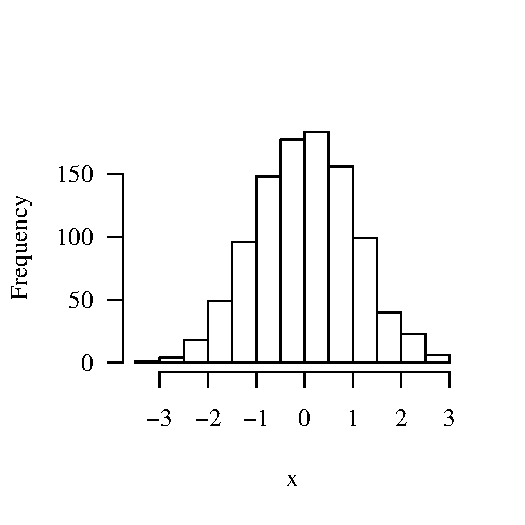
\includegraphics[width=4.6cm]{example_fig.pdf}
\begin{itemize}
\item Some insightful comment
\end{itemize}
\end{center}}

\end{minipage}

\end{frame}


\section{Section 2}

\subsection{Subsection title}
\begin{frame}

\begin{scriptsize}
\begin{table}[htp!]
\caption{A pretty table}
    \centering
\begin{tabular}{l | m{7mm} | c c }
\hline
&  & \textbf{Column A} & \textbf{Column B} \\
\hline
\parbox[t]{2mm}{\multirow{4}{*}{\rotatebox[origin=c]{90}{ \textcolor{red}{Super-group 1} }}} & \parbox[t]{2mm}{\multirow{2}{*}{\rotatebox[origin=c]{90}{\textbf{$\Gamma$}} \rotatebox[origin=c]{90}{\textbf{one}} }  } & A & B \\[1mm]
&  & C     & D \\[1mm]
\cline{2-4}
&  \parbox[t]{2mm}{\multirow{2}{*}{\rotatebox[origin=c]{90}{\textbf{$\Gamma$}} \rotatebox[origin=c]{90}{\textbf{two}} }}  & E & F \\[1mm]
& & G 		 & H \\[1mm]
\hline
\parbox[t]{2mm}{\multirow{4}{*}{\rotatebox[origin=c]{90}{ \textcolor{orange}{Super-group 2} }}} & \parbox[t]{2mm}{\multirow{2}{*}{\rotatebox[origin=c]{90}{\textbf{$\Delta$}} \rotatebox[origin=c]{90}{\textbf{one}} }  } & I & J \\[1mm] 
&  & K     & L \\[1mm]
\cline{2-4}
&  \parbox[t]{2mm}{\multirow{2}{*}{\rotatebox[origin=c]{90}{\textbf{$\Delta$}} \rotatebox[origin=c]{90}{\textbf{two}} }}  & M & N  \\[1mm]
& & O 		 &  P  \\[1mm]
\hline
\end{tabular}
\label{tab:estimates}
\end{table}
\end{scriptsize}


\end{frame}


\section*{}


\section*{Acknowledgments}
\begin{frame}

\small{
Thanks to Bob 
}


\begin{center}
\vspace{1cm}
\Large \textbf{Thank you for your attention.}
\vspace{5mm}
\end{center} 

\begin{flushright}
\begin{minipage}{0.45\linewidth}
This work was funded by ...
\end{minipage}
\end{flushright}

\end{frame}


\appendix

\begin{frame}
\bibliographystyle{IARC} 
\begin{tiny}  
\bibliography{example}         
\end{tiny}
\end{frame}


\section{SI}

\begin{frame}
\label{SI1}

\textbf{Backup slides}

\end{frame}


\end{document}
